
\documentclass[conference,final,12pt,]{IEEEtran}


\ifCLASSINFOpdf

\else
\texttt{new times roman}
\fi



\usepackage{graphicx}

\makeatletter
\def\maxwidth{\ifdim\Gin@nat@width>\linewidth\linewidth
\else\Gin@nat@width\fi}
\makeatother
\let\Oldincludegraphics\includegraphics
\renewcommand{\includegraphics}[1]{\Oldincludegraphics[width=\maxwidth]{#1}}

\usepackage[unicode=true]{hyperref}
\usepackage[spanish]{babel}
\usepackage[utf8]{inputenc} 
\usepackage[T1]{fontenc}
%\usepackage{newtxmath,newtxtext}
\usepackage{bookman}
\usepackage{lmodern}
\usepackage{natbib}
\bibliographystyle{jss}
\renewcommand{\spanishtablename}{Tabla}

\hypersetup{
            pdftitle={Bare Demo of IEEEtran.cls for IEEE Conferences},
            pdfkeywords={Diversidad, Zonación, Similitud, Manglar, Bosque aluvial},
            pdfborder={0 0 0},
            breaklinks=true, 
            colorlinks,
            citecolor=red,
            urlcolor=blue}
\urlstyle{same}  % don't use monospace font for urls

% Pandoc toggle for numbering sections (defaults to be off)
\setcounter{secnumdepth}{0}

% Pandoc syntax highlighting


% Pandoc header

\providecommand{\tightlist}{%
  \setlength{\itemsep}{0pt}\setlength{\parskip}{0pt}}

%% END MY ADDITIONS %%


\hyphenation{op-tical net-works semi-conduc-tor}

\begin{document}



\title{Comparación de la diversidad de tres parcelas y los cambios que presentan en sus estructuras en un bosque de manglar y un bosque aluvial de la costa del Urabá Antioqueño}


\author{

\IEEEauthorblockN{
  %% -- beg for/affiliation.institution.author
Cristian Gañan T %% -- end for/affiliation.institution.author
}
\IEEEauthorblockA{Dep. Ciencias Forestales\\
U Nacional de Colombia\\
Medelín, Antioquia
\\ccganant@unal.edu.co
}
\and
\IEEEauthorblockN{
  %% -- beg for/affiliation.institution.author
Camilo Cruz S %% -- end for/affiliation.institution.author
}
\IEEEauthorblockA{Dep. Ciencias Forestales\\
U Nacional de Colombia\\
Medellín, Antioquia
\\cacruzs@unal.edu.co
}
\and
\IEEEauthorblockN{
  %% -- beg for/affiliation.institution.author
Juan Caicedo G %% -- end for/affiliation.institution.author
}
\IEEEauthorblockA{Dep. Ciencias Forestales\\
U Nacional de Colombia\\
Medellín, Antioquia
  %% -- beg for/affiliation.institution.author
\\jpcaicedog@unal.edu.co
 %% -- end for/affiliation.institution.author
}
 
}



% use for special paper notices
%\IEEEspecialpapernotice{(Invited Paper)}




% make the title area
\maketitle

% As a general rule, do not put math, special symbols or citations
% in the abstract
\begin{abstract}
La diversidad es uno de los parámetros más importantes que se usan
para entender la dinámica de los ecosistemas y como está afecta a la
estructura de los bosques, a partir de esto se analizó la diversidad y
el cambio en las estructuras de 3 parcelas circulares (62, 69 y 70) de
\(500 \ m^2\), ubicadas en el Urabá Antioqueño, con el fin de
identificar si hacen parte de la misma comunidad o no; se utilizaron los
índices de diversidad alfa y beta, y diferentes modelos como de riqueza
esperada, de Valor de Importancia y diámetricos. Según los resultados de
los índices alfa se pudo llegar a la conclusión de que la parcela 69
tiene la mayor diversidad por las pruebas de Shannon, Simpson y Alfha;
de igual forma se encontró que la parcela 69 es diferente a las parcelas
62 y 70 por medio de los índices beta (Morisita y Sorensen), por lo
tanto se podría pensar que existe una zonación a través de las 3
parcelas, ubicando a la 62 y 70 más cercanas a la costa. Además se
determinó que la especie con más peso en el índice de valor de
importancia para las tres parcelas fue \emph{Rhizophora Mangle}. Adicionalmente
se realizaron modelos de distribución diamétrica ajustando para la
mayoría de las parcelas un modelo tipo ``gamma'' excepto la parcela 70
que se comportó mejor como ``weibull''.
\end{abstract}

% keywords
\begin{IEEEkeywords}
Diversidad; Zonación; Similitud; Manglar; Bosque Aluvial
\end{IEEEkeywords}

% use for special paper notices



% make the title area
\maketitle

% no keywords

% For peer review papers, you can put extra information on the cover
% page as needed:
% \ifCLASSOPTIONpeerreview
% \begin{center} \bfseries EDICS Category: 3-BBND \end{center}
% \fi
%
% For peerreview papers, this IEEEtran command inserts a page break and
% creates the second title. It will be ignored for other modes.
\IEEEpeerreviewmaketitle


\hypertarget{introducciuxf3n}{%
\section{Introducción}\label{introducciuxf3n}}

Los estudios de diversidad han sido catalogados desde el punto de vista
científico como una gran ayuda para entender la dinámica de los
distintos ecosistemas, también como sinónimo de ``variedad de vida''
\citep{A}. Existen dos áreas principales en las cuales los estudios y
medidas de diversidad han tenido una gran aplicación, se pueden ver
desde el punto de vista de la conservación la cual está basada
en que las comunidades ricas en especies son mejores que las pobres, y
desde el punto de vista de la supervisión ambiental, donde se tienen en
cuenta los efectos adversos en la reducción de la diversidad o en un
cambio de forma de la distribución de abundancia de las especies
\citep{B}. En los agrosistemas mantener o restaurar altos niveles de
diversidad, aumenta su resistencia al cambio climático, apoya la
provisión equilibrada de servicios ecosistémicos y contribuye a la
conectividad del hábitat \citep{C}.

La diversidad como una medida tangible es obtenida por medio de diversos
índices que además de dar un valor en cualquier comunidad, también
expresa comportamientos en las comunidades tales como la riqueza,
dominancia, equidad, abundancia relativa, similitud y disimilitud, entre
otros; los cuales son importantes de conocer, ya que pueden decir que
tan resistente sería la comunidad a periodos de tensión como
hídricos, de temperatura, enfermedades o cualquier otra causada de forma
natural o antrópica \citep{D}. Por otra parte, \citep{E} formalizó
matemáticamente el concepto de diversidad de especies y planteó tres
componentes cuantificables: alfa (\(\alpha\)), beta (\(\beta\)) y gamma
(\(\gamma\)), los cuales son importantes a la hora de querer conocer y
diferenciar la diversidad y estructura de distintas comunidades. Para este 
caso se tendrán en cuenta dos; los índices alfa cuantifican la diversidad dentro de una comunidad ( parcela), los beta la comparan entre varias comunidades y corrobora el reemplazamiento de especies entre una y otra \citep{G}.

La importancia de la determinación de los diferentes índices, está en
diferenciar entre tipos de bosques y conocer los cambios ambientales
para explicar el reemplazamiento de especies y el cambio en la
estructura, la cual está relacionada con la diversidad, pero también con
condiciones ambientales como el clima, el suelo\citep{H} y las exigencias
de las especies \citep{J} que hacen que esta cambie continuamente
\citep{I}; lo que da una idea acerca de qué tan diversos son y cual de
ellos representa una mayor complejidad estructural, teniendo en cuenta
los factores bióticos y abióticos que la controlan. La
estructura observada en cada situación particular es la mejor respuesta
del ecosistema a sus propias características \citep{F}.

En este artículo se tiene como objetivo comparar la diversidad entre
parcelas que vienen de dos tipos de bosques en el Urabá Antioqueño
(manglares y bosques inundables) y cómo esta afecta la configuración de
la comunidad y si las diferentes parcelas pertenecen a una misma
comunidad o no, todo esto con la ayuda de los diferentes índices de
diversidad y componentes de la estructura. Además de análisis como el
índice de valor de importancia(IVI), que ayuda a cuantificar la
relevancia de las diferentes especies en las parcelas y otros que
permiten comparar y entender la zonación, es decir, el cambio que
presentan las especies más importantes a lo largo de un gradiente de 
condiciones ambientales, teniendo en cuenta las preferencias ecológicas
de dichas especies.

\hypertarget{materiales-y-muxe9todos}{%
\section{Materiales y métodos}\label{materiales-y-muxe9todos}}

Las parcelas que se comparan en el presente estudio fueron tomadas de
una base de datos realizada por \citep{AB} pertenecientes a dos tipos de
bosques (Manglares y bosques Aluviales) en el Urabá Antioqueño, con el
fin de determinar la variabilidad de la vegetación a lo largo de las
costas, por medio de la evaluación de la estructura, composición
florística y atributos ambientales de los manglares. Según los autores
el trabajo de campo se realizó de septiembre de 2009 a enero 2010, y se
trazaron 87 parcelas circulares de \(500 \ m^2\). Se midió el diámetro a la
altura del pecho (DAP) y altura total de todos los árboles con DAP
superior a 5 cm en cada parcela, y se identificó cada individuo con DAP
entre 2.5 y 5 cm. Además se tomaron datos de salinidad e inundación de
cada parcela. En este artículo solo se tendrán en cuenta las parcelas
62, 69 y 70, para la cuales se hallaron índices de diversidad Alfa y
Beta con el fin de compararlas. Para el cálculo de la diversidad alfa se
utilizaron los índices de Shannon, Simpson (1-D), alfa de Fisher y el
índice de riqueza de Margalef y para el cálculo de diversidad Beta se
usaron los índices de Sorensen y Morishita. Adicionalmente se calculó la
riqueza esperada por medio del modelo de Jacknife y rarefacción, también
se calculó el número efectivo de especies por medio la fórmula propuesta
por Jost y finalmente para entender el comportamiento de la estructura
se calculó el IVI suponiendo que las tres parcelas estan en una sola comunidad y
se hallaron modelos de distribución diamétrica. Todos los Cálculos
fueron realizados a través del software R versión 3.6.1

\textbf{Índices de diversidad alfa.}Las medidas de diversidad más
ampliamente usadas son los índices de la teoría de la información. Estos
se basan en la lógica de que la diversidad en un
sistema natural pueden ser medidos de un modo similar a la información
contenida en un código o mensaje. Algunos de estos índices 
son los de Shannon y Simpson \citep{B}.

\textbf{Shannon y Simpson.}El índice de Shannon
refleja la heterogeneidad de una comunidad sobre la base de dos
factores: el número de especies presentes y su abundancia relativa. La
diversidad máxima (Hmax= lnS) se alcanza cuando todas las especies están
igualmente presentes \citep{L}. El Índice de Simpson es una medida de dominio,
pero también puede ser convertido en medida de diversidad restándole a
su resultado 1, este se puede establecer como la probabilidad de que dos
individuos tomados al azar de una comunidad sean de diferente especie, entonces el
criterio de diversidad está determinado por el número de pares de
individuos que difieren en especie \citep{M}.

\textbf{Margalef.}El índice de riqueza de Margalef transforma el número de
especies por muestra a una proporción en las cuales son añadidas por
expansión de la muestra \citep{N}, es decir, a mayor intensidad de muestreo
se espera mayor riqueza de especies. Cuando el índice arroja un resultado 
de cero indica que solo existe una especie en la
muestra \citep{N}. 

\textbf{Alfa de Fisher.}Es un modelo de abundancia a partir de una serie logarítmica que solo toma
en cuenta el número de especies (S) y el número total de individuos(N)
\citep{P}. Este índice funciona mejor con datos donde todas las especies
tienen una baja abundancia \citep{Q}. El alfa de Fisher es una
herramienta muy eficaz para estimar la magnitud de las diferencias
esperadas en términos de la riqueza entre regiones con tamaños de
muestra más grandes, con base en un número limitado de individuos.
\citep{R}. Para este caso se tomó un total de 100.

\textbf{Índices beta.} El concepto de diversidad \(\beta\) tiene gran relevancia
en ecología y biogeografía para comprender, cuantificar y valorar la
diversidad biológica, el funcionamiento de los ecosistemas, la conservación de la biodiversidad y el manejo de estos \citep{O}, \citep{AP} la define
como ``la magnitud de cambio en la composición de las especies a lo
largo de un gradiente ambiental o entre diferentes comunidades en un
paisaje''. La forma más sencilla de medir la diversidad Beta es mediante
el uso de coeficientes de similaridad \citep{B}, entre estos se pueden
encontrar los índices de Sorensen y Morisita-Horn, que son medidas
cuantitativas que tienen en cuenta la abundancia relativa.

\textbf{Riqueza esperada.}Cuando se hacen inventarios forestales con el
fin de determinar la biodiversidad de algún tipo de sistema, siempre se
tiene el problema de no muestrear la cantidad total de especies que se
pueden encontrar en dicho espacio, y al mismo tiempo para poder comparar
entre comunidades se necesitan las mismas muestras en ambos sitios, por
lo tanto la rarefacción se impuso como un método ampliamente utilizado
\citep{Z}, por otra parte los métodos no paramétricos como el Jacknife
\citep{AA} para dar solución a este problema y determinar la riqueza
esperada de algún lugar en estudio.

\textbf{Jacknife.} Modelo usado para la estimación de la riqueza \citep{X}, se
basa en el número de especies raras, existen dos modelos Jack 1 y Jack
2, para este estudio se usa solo Jack 1 que tiene en cuenta el número de
especies raras presentes en una sola unidad de muestreo \citep{Y} 

\textbf{Rarefacción.} Es un método que se usa para obtener las especies
esperadas. Se estima en base a un numero estandar de muestras, es decir,
teniendo en cuenta que todas las comunidades tuvieran el mismo número de
individuos \citep{B}, para este estudio se toman 30, debido a
que fue este el número mínimo de muestreo de las 3 parcelas, perteneciente
a la parcela 70.

\textbf{Número efectivo de especies.} Permiten obtener una interpretación
intuitiva y fácilmente comparable de la diversidad\citep{V};
desde el enfoque de la ecología, puede definirse como el
recíproco de un promedio de las abundancias relativas de las especies,
el valor de este recíproco es el número máximo posible de estas que
podrían coexistir en una comunidad si todas tuvieran la misma
abundancia \citep{W}. Se halla con la fórmula propuesta por Jost, que
cambia según el valor del parámetro q; este determina qué tanto influyen las
especies comunes o raras en la medida de la diversidad, y
puede tomar cualquier valor que el usuario estime apropiado. Si q=0 el
valor de la ecuación equivale a la riqueza de especies, si q=1 es
equivalente al exponencial del índice de Shannon y si q=2 es
equivalente al índice de dominancia de Simpson \citep{AV}.

\textbf{Medidas para entender el comportamiento de la estructura.} \\
\emph{Índice de valor de importancia.} Desarrollado por 
\cite{T}, es un índice que permite comparar el peso o valor ecológico
relativo de las especies dentro de la comunidad y consiste en la
sumatoria de los valores relativos de densidad, frecuencia y
dominancia \citep{U}. Se asumió una sola comunidad entre las tres
parcelas para este índice.

\emph{Modelos de distribución diamétrica.} Las distribuciones
diamétricas son las relaciones del diámetro con sus frecuencias absolutas, 
estas tienen aplicabilidad en varios campos, son muy útiles para la caracterización de  las diferentes interacciones entre especies, así como irregularidades debidas a la historia del bosque, la geomorfología, topografía y al comportamiento de algunas especies \citep{AE}, en este sentido, se eligieron algunos de los
modelos más conocidos para ajustar los datos, estos fueron: Weibull y
Gamma.

\hypertarget{resultados-y-discusiuxf3n}{%
\section{Resultados y discusión}\label{resultados-y-discusiuxf3n}}

\textbf{Índices alfa} 

En la \textbf{Tabla I} se pueden observar los
resultados de los diferentes índices para la diversidad alfa. En el
índice de Margalef se ve que las tres parcelas tienen una
baja riqueza de especies, ya que cuentan con un valor por debajo de 2
\citep{B},sin embargo al compararlas, la parcela 69 es la de mayor
diversidad; esta tendencia a presentar baja riqueza era de
esperarse, ya que son comunidades que tienen unas restricciones
ambientales importantes, sea por la salinidad en los manglares
\citep{AD} o por los periodos de inundación a los que se ven sometidos
los bosques aluviales \citep{Z}; en este caso se puede evidenciar con los
datos, que la parcela 62 tiene una riqueza muy baja
y una diversidad dada por el índice de simpson igualmente baja, esto es
debido a la alta presencia y dominancia de la especie \emph{Rhizophora
Mangle}, que según \citep{Z}, en los manglares esta es la especie mejor
conocida, por lo tanto se puede pensar que la parcela hace referencia
a un bosque que posiblemente está más cerca a la costa y se podría
catalogar como manglar.

\begin{table}[htb]

\caption{\label{tab:unnamed-chunk-2}indices alfa}
\centering
\begin{tabular}[t]{l|r|r|r|r}
\hline
Parcela & Margalef & Shannon & Simpson & Fisher\\
\hline
62 & 0.22 & 0.062 & 0.022 & 2.043\\
\hline
69 & 1.15 & 1.15 & 0.62 & 6.37\\
\hline
70 & 0.58 & 0.38 & 0.18 & 3.94\\
\hline
\end{tabular}
\end{table}

Teniendo en cuenta lo anterior y con la realización de los demás índices
de diversidad (Shannon, Simpson y alfa de Fisher)(\textbf{Tabla I}) se
puede verificar que la diversidad aumenta (sin ser alta), según el alfa
Fisher desde la parcela 62, que es la de más baja diversidad, hacia la
parcela 70 y terminando con la parcela 69, esto debido al mayor número
de especies y una dominancia no tan marcada en esta última, comprobando
así que entre el índice de alfa y el índice de dominancia de Simpson hay
una relación inversa, es decir, a mayor índice de diversidad alfa menor
índice de dominancia de simpson, la parcela 69 cuenta con el índice más
alto de alfa de Fisher(6.37) y el índice más bajo de dominancia de
Simpson(1-0.62=0.38) entre las tres parcelas. Lo que concuerda 
con \citep{Z} donde se dice que las comunidades más heterogéneas
de ecosistemas en contacto directo con el agua, se encuentran más
alejadas del mar. Se puede intuir que la parcela 69 es la
que está más alejada de la acción salobre del agua, algo que afirma esta
idea es la presencia de la especie \emph{Pterocarpus officinalis}, común 
en bosques inundables que no tienen contacto con el
efecto salobre del mar \citep{Y}, por ende, siendo la
más alejada de la costa se podría catalogar como bosque
aluvial o inundable.

\begin{table}[htb]

\caption{\label{tab:unnamed-chunk-3}Índices Beta}
\centering
\begin{tabular}[t]{l|r|r}
\hline
Comparación & Morisita-Horn (\%) & Sorensen\\
\hline
62 vs 70 & 99.44 & 0.8\\
\hline
69 vs 70 & 0.00 & 0.0\\
\hline
62 vs 69 & 0.00 & 0.0\\
\hline
\end{tabular}
\end{table}

\textbf{Índices Beta}

En la \textbf{Tabla II} se pueden observar los índices de diversidad
Beta, según esto la parcela 62 y 70 son muy similares, llegando a pensar
que son de la misma comunidad, ya que el índice de Morisita arroja un
resultado del 99.43 \(\%\) de similitud. Caso totalmente contrario pasa con
las comparaciones restantes(69 vs 70 y 62 vs 69) donde Morisita arroja
un valor del 0 \(\%\), lo que puede atribuirse a que entre
estas parcelas no hay especies en común. Se puede llegar a la misma
conclusión si se analiza el índice de Sorensen que se mide de 0 a 1
donde 0 indica que las parcelas no tienen ninguna similitud; para la
comparación entre la parcela 62 y 70 arroja un resultado de 0.80,
teniendo concordancia con el índice de Morisita; caso mismo ocurre en
las otras comparaciones donde el resultado es de 0. Con estos datos se
puede afirmar que la parcela 62 es igual a la 70 y que la parcela 69 es
totalmente diferente. Por lo tanto se concluye que las parcelas
70 y 62 hacen parte del manglar, ya que las
especies de la parcela 70 son comunes en estos,
incluyendo la especie \emph{Pelliciera rhizophorae} \citep{Y} que no se
encuentra en la parcela 62. Por último se confirma la idea de que la parcela
69 hace parte de un bosque aluvial, no solo por los resultados en los índices Beta,
si no también por las especies pertenecientes a dicha parcela 
(\emph{Prioria copaifera,  Tabebuia chrysantha, Pachira cf. aquatica  ,   
Raphia taedigera,  Montrichardia arborescens,  Pterocarpus officinalis})
que son comunes de un bosque aluvial \citep{Y}.

\begin{table}[htb]

\caption{\label{tab:unnamed-chunk-4}Índices de especies efectivas}
\centering
\begin{tabular}[t]{l|r|r|r}
\hline
Índice & Parcela 62 & Parcela 69 & Parcela 70\\
\hline
q= 0 & 2.00 & 6.00 & 3.00\\
\hline
q= 1 & 1.06 & 3.14 & 1.46\\
\hline
q= 2 & 0.97 & 0.37 & 0.82\\
\hline
\end{tabular}
\end{table}

Los resultados que se muestran en la \textbf{Tabla III}(Índice de
especies efectivas) permiten comparar riqueza, dominancia y diversidad
\citep{V}. Observando los resultados, se puede evidenciar que la
tendencia de los diferentes índices en las parcelas siguen el mismo
orden discutido anteriormente con los alfa (\textbf{Tabla I}), que
también ubican a la parcela 62 con la mayor dominancia y a la parcela 69
como la más diversa. La diferencia más representativa entre los dos
tipos de índices es cuando el parámetro q en la fórmula de especies
efectivas es igual a 1 que hace referencia al exponencial de shannon,
este valor explica las especies necesarias para alcanzar un índice de
diversidad de Shannon dado \citep{B}. La parcela 69 tiene el índice
de diversidad de shannon más alto (1.15), valor que podría alcanzarse con
tan solo 4 especies, por lo cual se podría decir que dos de las seis
especies están muy poco representadas en la parcela (\emph{Prioria
copaifera} y \emph{Tabebuia chrysantha}). Con el índice de especies
efectivas se puede intuir que a través de las tres parcelas se presenta
una zonación que va desde la parcela 62, siendo ésta bosque de manglar,
seguida de la parcela 70 y finalmente la parcela 69 la cual se clasificó
como bosque aluvial. Conclusiones a las cuales ya se habían llegado
anteriormente.

\begin{figure}[htb]
\centering
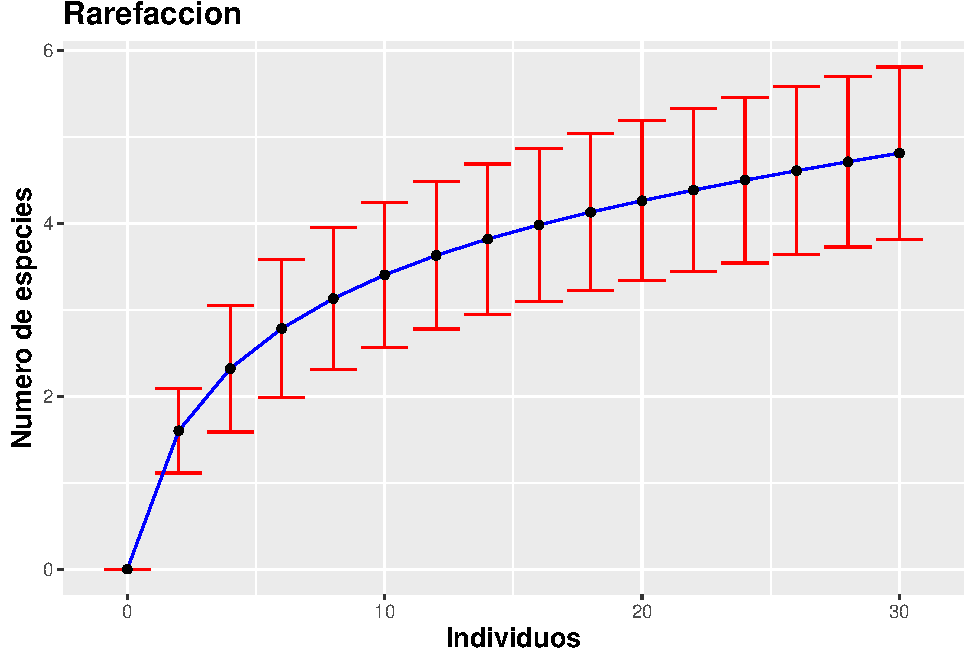
\includegraphics{mangrove_files/figure-latex/unnamed-chunk-5-1.pdf}
\caption{Rarefacción por Parcela}
\end{figure}

\textbf{Rarefacción} 

En la \textbf{figura 1} se puede encontrar las
curvas de rarefacción por separado de las 3 parcelas en estudio, donde
se observa que la 62 y 70 muestran una tendencia más cercana a una
asíntota horizontal; dado que el método permite la comparación de la
riqueza de especies entre los conjuntos de datos \citep{AM} y que las
estimaciones de riqueza de especies aumentan con el número de unidades
de muestreo \citep{AN}, se puede intuir que por la alta dominancia de
estas parcelas, el número máximo de especies esperadas está muy cercano
al observado, además es probable que como se encuentran en un entorno de
salinidad considerable sean comunidades con condiciones ambientales
especiales, es decir, al extremo de un gradiente ambiental; lo que no
sucede en la parcela 69 donde la curva está aún en un comportamiento de
alta pendiente, que sugiere más muestreos para alcanzar el máximo número
de especies esperadas, también la mayor heterogeneidad que se presenta en la
parcela indicaría que no se encuentra al extremo de un gradiente. Esto
refleja que la disposición de especies a lo largo de una variación
ambiental, tienen un óptimo ecológico \citep{AO}.

\begin{figure}[htb]
\centering
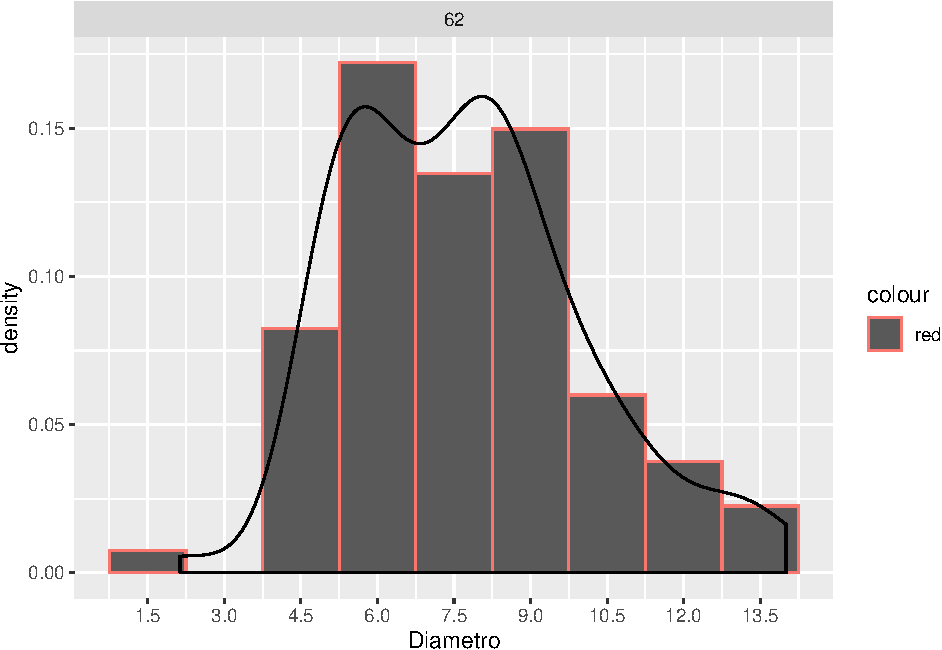
\includegraphics{mangrove_files/figure-latex/unnamed-chunk-6-1.pdf}
\caption{Rarefacción}
\end{figure}

En la \textbf{figura 2} se muestra el comportamiento de la curva de
rarefacción de la comunidad; se evidencia que se debería
muestrear más para que esta alcance su asíntota (número máximo esperado
de especies), la figura también indica que con un muestreo de 30
individuos se espera encontrar entre 4 y 5 especies, idea que podría ser
explicada por lo dominancia tan marcada en las parcelas
62 y 70, que hacen que la curva tienda a menos especies, recordando que
el número total de especies muestreadas fue de 9. Según la aplicación
del método de Jacknife se podrían esperar un total de 14 especies para
toda la comunidad, número muy diferente al encontrado con el
método anterior. 

Dado que la rarefacción basada en individuos, genera
una importante pérdida de la información, por la toma de un tamaño
general para todas las muestras basado en el tamaño de muestra más
pequeño\citep{AQ} y que el método de Jacknife, que suele ser estable con
tamaños de muestras pequeños \citep{AS} y además ha sido catalogado por
varios estudios \cite{AS,AT,AU} como el menos sesgado y
más exacto, se cree que la probabilidad de encontrar el mejor resultado
para el número total de especies esperadas, sería por medio del método de
Jacknife.

\begin{table}[htb]

\caption{\label{tab:unnamed-chunk-7}Índice de valor de importancia}
\centering
\begin{tabular}[t]{l|r|r}
\hline
Especie & DR & IVI\\
\hline
Prioria copaifera & 0.07 & 9.67\\
\hline
Pelliciera rhizophorae & 0.16 & 9.75\\
\hline
Tabebuia chrysantha & 0.21 & 9.81\\
\hline
Pachira cf. aquatica & 4.52 & 17.15\\
\hline
Raphia taedigera & 7.12 & 17.22\\
\hline
Laguncularia racemosa & 1.93 & 21.62\\
\hline
Montrichardia arborescens & 6.96 & 33.73\\
\hline
Pterocarpus officinalis & 41.51 & 66.76\\
\hline
Rhizophora mangle & 37.52 & 114.28\\
\hline
\end{tabular}
\end{table}

\textbf{Índice de valor de importancia}

En la \textbf{Tabla IV} se muestra el IVI para la comunidad, 
organizado en orden ascendente. Colocando a la especie \emph{Rhizophora Mangle} como la más importante. Las otras
2 especies más importantes según el IVI fueron: \emph{Pterocarpus
Officinalis} y \emph{Montrichardia arborescens}. Si se organizara en una
zonación a estas tres especies según sus preferencias ecológicas, seria:
primero empezando con \emph{Rhizophora Mangle} que tiene una mayor
dominancia en las parcelas 62 y 70, las cuales presentan unas
condiciones de salinidad de 2.2 y 4.6 ppm respectivamente, y ausencia
de la especie en la parcela 69. Esto puede deberse a que esta especie
soporta ambientes con alta salinidad e inundación \citep{AF}, y presenta
adaptaciones a estas condiciones, como las raíces fúlcreas, presencia de
neumatóforos \citep{AF} y lenticelas en las raíces para el intercambio
gaseoso. Segundo, avanzando en el paisaje, se encuentra que
\emph{Pterocarpus Officinalis} tiene una mayor dominancia en la parcela
69 que cuenta con un nivel de salinidad de 0.8 ppm, esta especie es un
árbol de hoja perenne de contrafuerte grande y relativamente tolerante a
la sal \citep{AG}, según \citep{AH} es particularmente vulnerable al
aumento de la salinidad, pues incrementa las tasas de mortalidad de
adultos al tiempo que reduce el crecimiento y reclutamiento;
finalmente \emph{Montrichardia arborescens}, que a pesar de que su
dominancia relativa (6.9) es baja respecto a las otras dos especies
mencionadas anteriormente, es la tercera especie más importante de la
comunidad, lo que puede darse a que esta habita en ambientes con
inundaciones temporales y baja influencia del mar (poca salinidad), esta especie presenta adaptaciones
morfologicas y fisiologicas que le permiten crecer en las condiciones de
la parcela 69 \citep{AI} (baja salinidad e inundación moderada). Se puede ver que los diferentes tipos de salinidad de las parcelas explican la
distribución de las especies y se confirma una zonación en la comunidad,
que va desde las parcelas 70 y 62 hacía la 69; ya que unas especies están
adaptadas a ambientes más salinos (las de las parcelas 62 y 70) y otras
están adaptadas a lugares con una salinidad baja (las de la parcela 69).

\begin{figure}[htb]
\centering
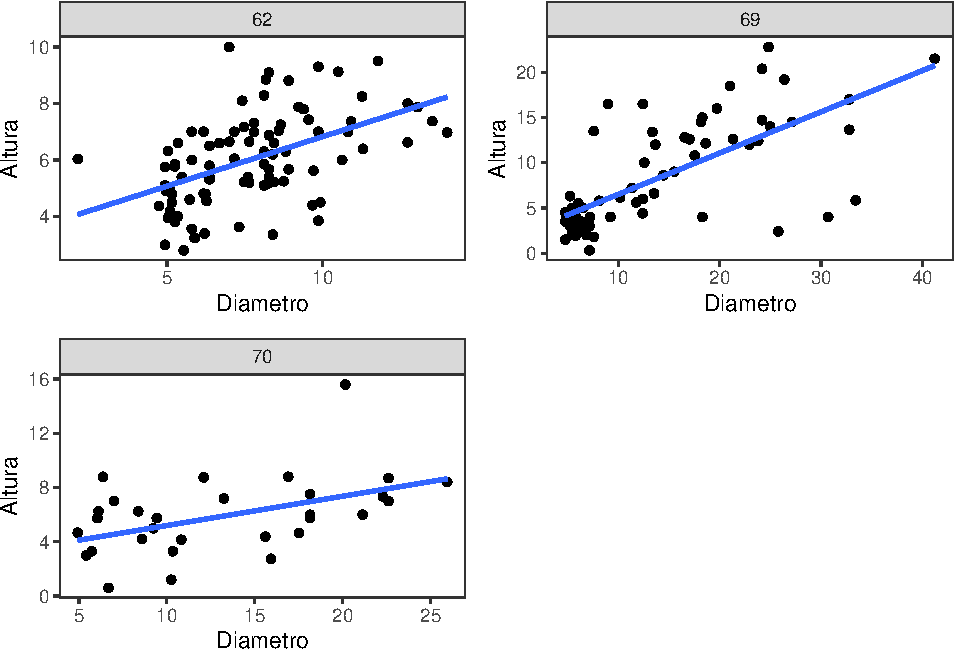
\includegraphics{mangrove_files/figure-latex/unnamed-chunk-14-1.pdf}
\caption{Relación diametro altura en las tres parcelas}
\end{figure}

\begin{figure}[htb]
\centering
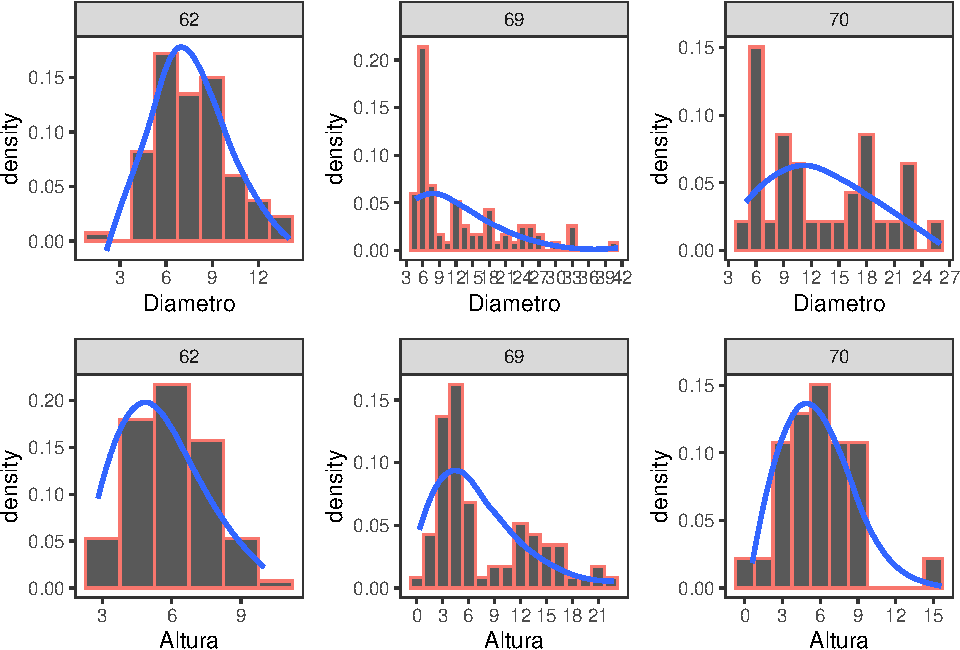
\includegraphics{mangrove_files/figure-latex/unnamed-chunk-15-1.pdf}
\caption{Distribuciónes diamétricas y de alturas}
\end{figure}

\textbf{Distribuciones diamétricas y de alturas}

En la \textbf{figura 4} se muestran las distribuciones de diámetro (D) y
altura (A). Todas las parcelas ajustaron a un modelo tipo ``gamma''
excepto la parcela 70 que se comportó mejor como ``weibull'' para ambos
casos. Es evidente notar que hay alturas y diámetros pequeños para todas
las parcelas, sin embargo hay ciertos valores variables que sugieren
diferentes tipos de regeneración, donde la más temprana se presenta en
la parcela 62, pues hay una acumulación en los rangos de 6 a 9 cm para D
y unos pocos son más grandes, algo parecido ocurre con la A, esto quiere
decir que el comportamiento es parecido a un bosque
coetáneo común en plantaciones \citep{AL}, lo que puede atribuirse a la
gran dominancia de \emph{Rhizophora Mangle}, si bien no es una
plantación, las características de dominancia hace que el comportamiento
en cuanto a D y A sean parecidos; la misma situación ocurre en la parcela
70, pero acá el patrón es más evidente en la distribución de A, parece
ser que en este punto de regeneración hay una preferencia de las
especies por aumentar de diámetro que en altura (\textbf{figura 3}), lo
que podría indicar que no hay competencia por luz, pues la estructura
del dosel está correlacionada con la luz del sotobosque \citep{AK} y ya
que hay una gran dominancia no habría una gran competencia
interespecífica. La tendencia descrita anteriormente no se cumple con la
parcela 69, pues acá hay más variabilidad en los parámetros de altura y
diámetro, lo que puede indicar la formación de estratos (agrupación de
puntos al principio de la gráfica)( \textbf{figura 3}) es notable la
asimetría positiva que presentan las distribuciones, muy propias de un
modelo ``gamma'' \citep{AJ}, la poca frecuencia que tienen los tamaños
grandes indica que hay acceso a la luz para todas las especies, lo que
precisamente hace pensar que hay en el estratos bosque, muchos árboles
pequeños y unos pocos altos o emergentes. Según esto, es posible intuir
que a mayor dominancia de una especie, la probabilidad de encontrar
estratos en el bosque será menor.


\bibliography{mybibfile}

\end{document}


